\chapter{Basic Techniques}\label{chap:basic-theory}

The Subgraph Enumeration algorithm can be decomposed into three major steps: (1) Query Graph Preprocessing, (2) Data Graph Preprocessing, and (3) Search Tree Traversal. This chapter covers each step in detail with a running example.

\begin{figure}
    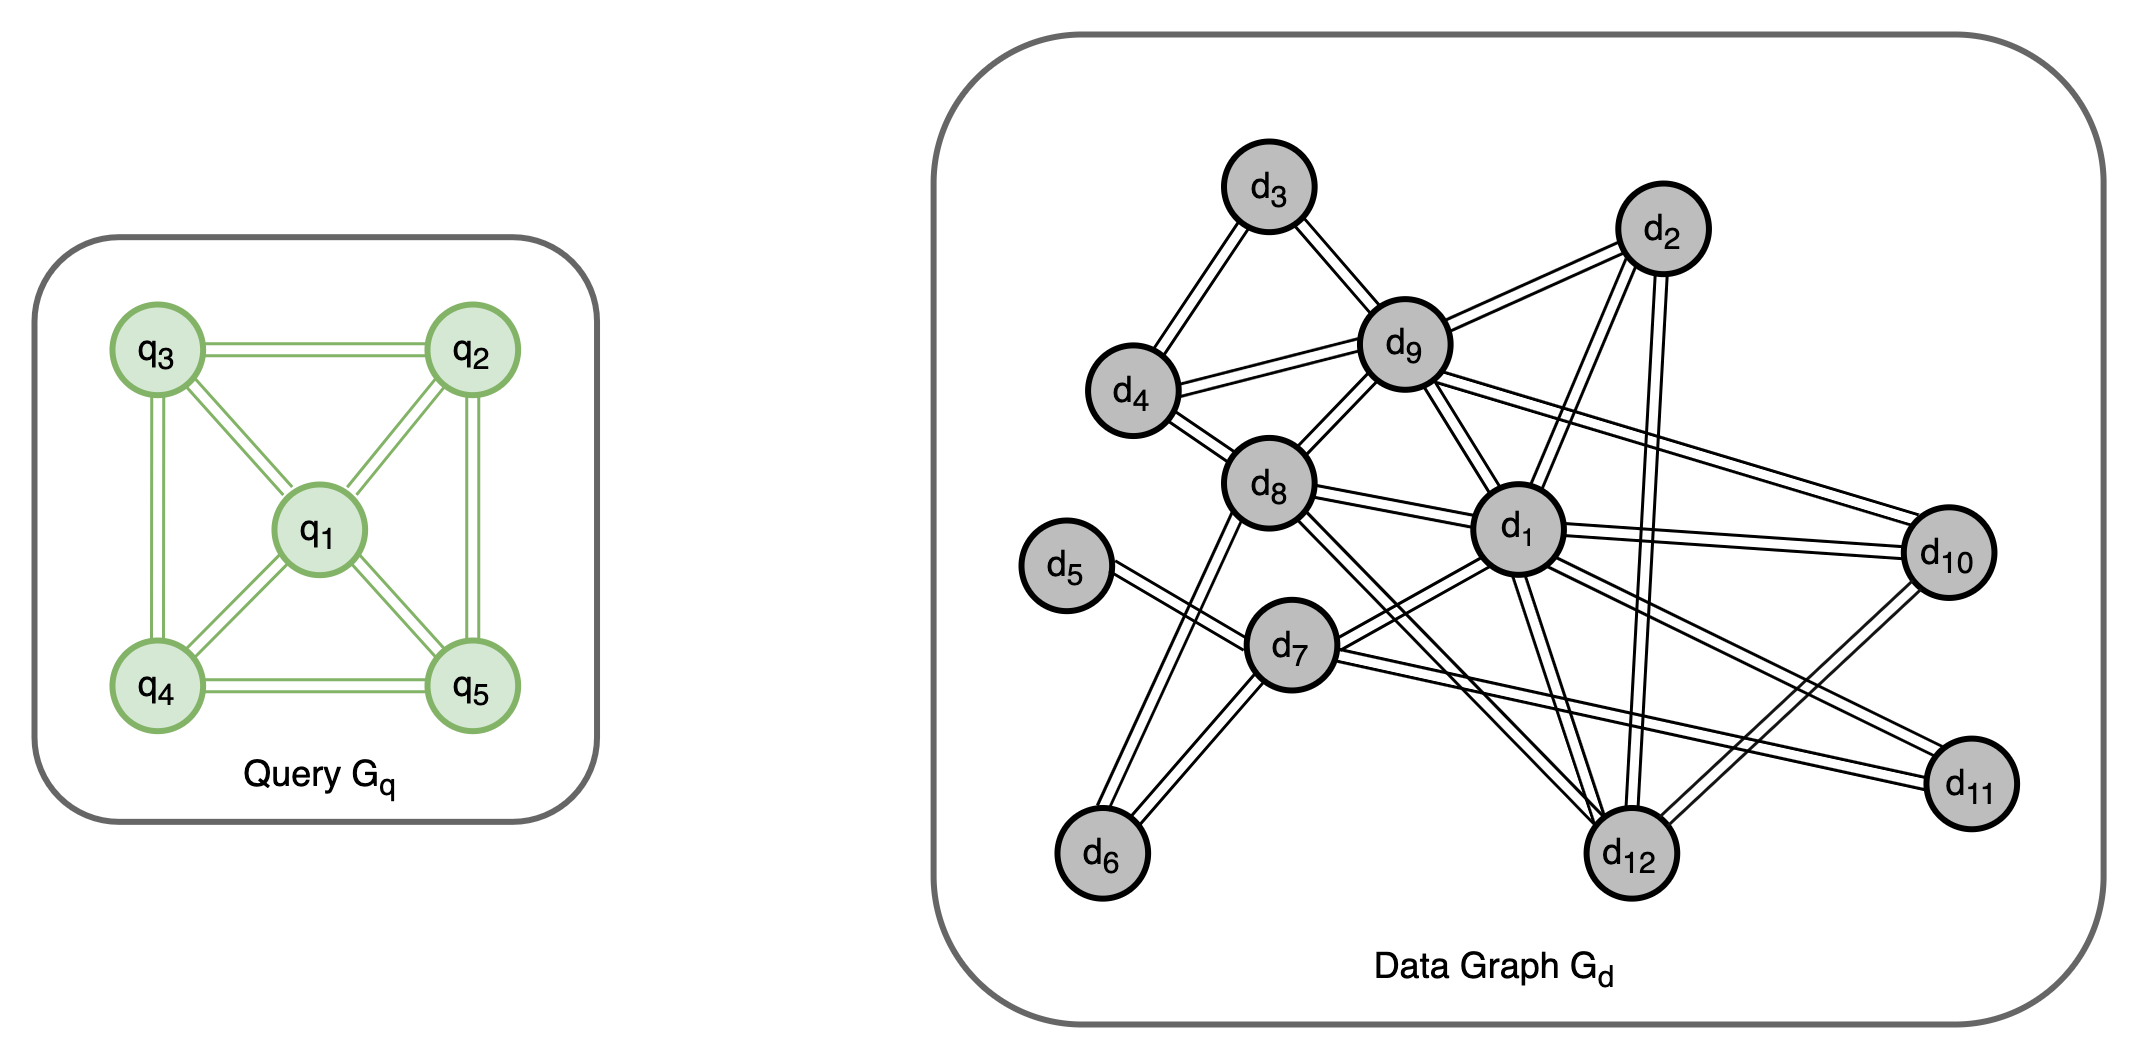
\includegraphics[width=\textwidth]{fig/LR/sgm-example1.png}
    \caption{Example}
    \label{fig:sgm-example}
\end{figure}
\section{Query Graph Preprocessing}\label{query-preprocessing}
This section explains all processing done on the query graph to enable it for search tree traversal.
% The main tasks performed on the input query are Query sequencing and Symmetry Detection.
\textit{Query sequencing} and \textit{Symmetry Detection} are the main tasks performed on the input query.
Since the query graphs are very small and all preprocessing tasks are polynomial time complexity, this preprocessing workload is handled by the CPU.
Query preprocessing is important to shrink the search tree exploration, the amount of work done at each node, and redundancy elimination.

\subsection{Query Sequencing}
The query graph input to the application is undirected. The first task is to convert this undirected graph to a directed acyclic graph (DAG). The ordering of the DAG governs the order in which these vertices are matched to the data graph.
The query nodes are ordered based on their likelihood of matching with the data graph. Naturally, query nodes with lesser likelihood are prioritized over others.

The query sequencing algorithm used by VF3 \cite{VF3} is utilized for this task. This algorithm uses multiple criteria to estimate the likelihood of matching and sequences the nodes in decreasing order of that likelihood.
Interested readers are encouraged to read about these criteria in \cite{VF3}.
The pseudocode is listed in Algorithm \ref{algo:query-seq}.
The order generated after performing query sequencing on the do graph is shown in Figure \ref{fig:query-sequencing}.

\begin{algorithm}[h]
    \caption{Query Sequencing}
    \label{algo:query-seq}

    \SetKwData{dm}{$d_M$}
    \SetKwData{deg}{Degree}
    \SetKwData{lh}{likelihood}
    \SetKwData{i}{i}
    \SetKwData{j}{j}
    \SetKwData{idx}{idx}
    \SetKwData{seq}{$S_q$}

    \SetKwFunction{argmax}{argmax}

    \KwIn{Template Graph, $G_q$}
    \KwOut{Node Query Sequence, $S_q$}
    $\dm[N_q] \leftarrow 0$\;
    $S_q \leftarrow \phi$\;
    \For{$\i \leftarrow$ 0 \KwTo $N_q$}{
        \tcp{calculate likelihood for remaining nodes}
        \For{$\j \leftarrow 0$ \KwTo $N_q$}{
            \If{\j not in \seq } {
                $\lh[\j] \leftarrow \dm[\j] \times N_q + \deg[\j]$\;
            }
        }
        \tcp{Find node with maximum likelihood and it to \seq}
        \idx $\leftarrow$ \argmax{\lh}\;
        append \idx to \seq\;

        \tcp{Update \dm}
        \ForEach{neighbor \j of node \idx}{$\dm[\j] \leftarrow \dm[\j] + 1$\;}
    }
\end{algorithm}



\begin{figure}
    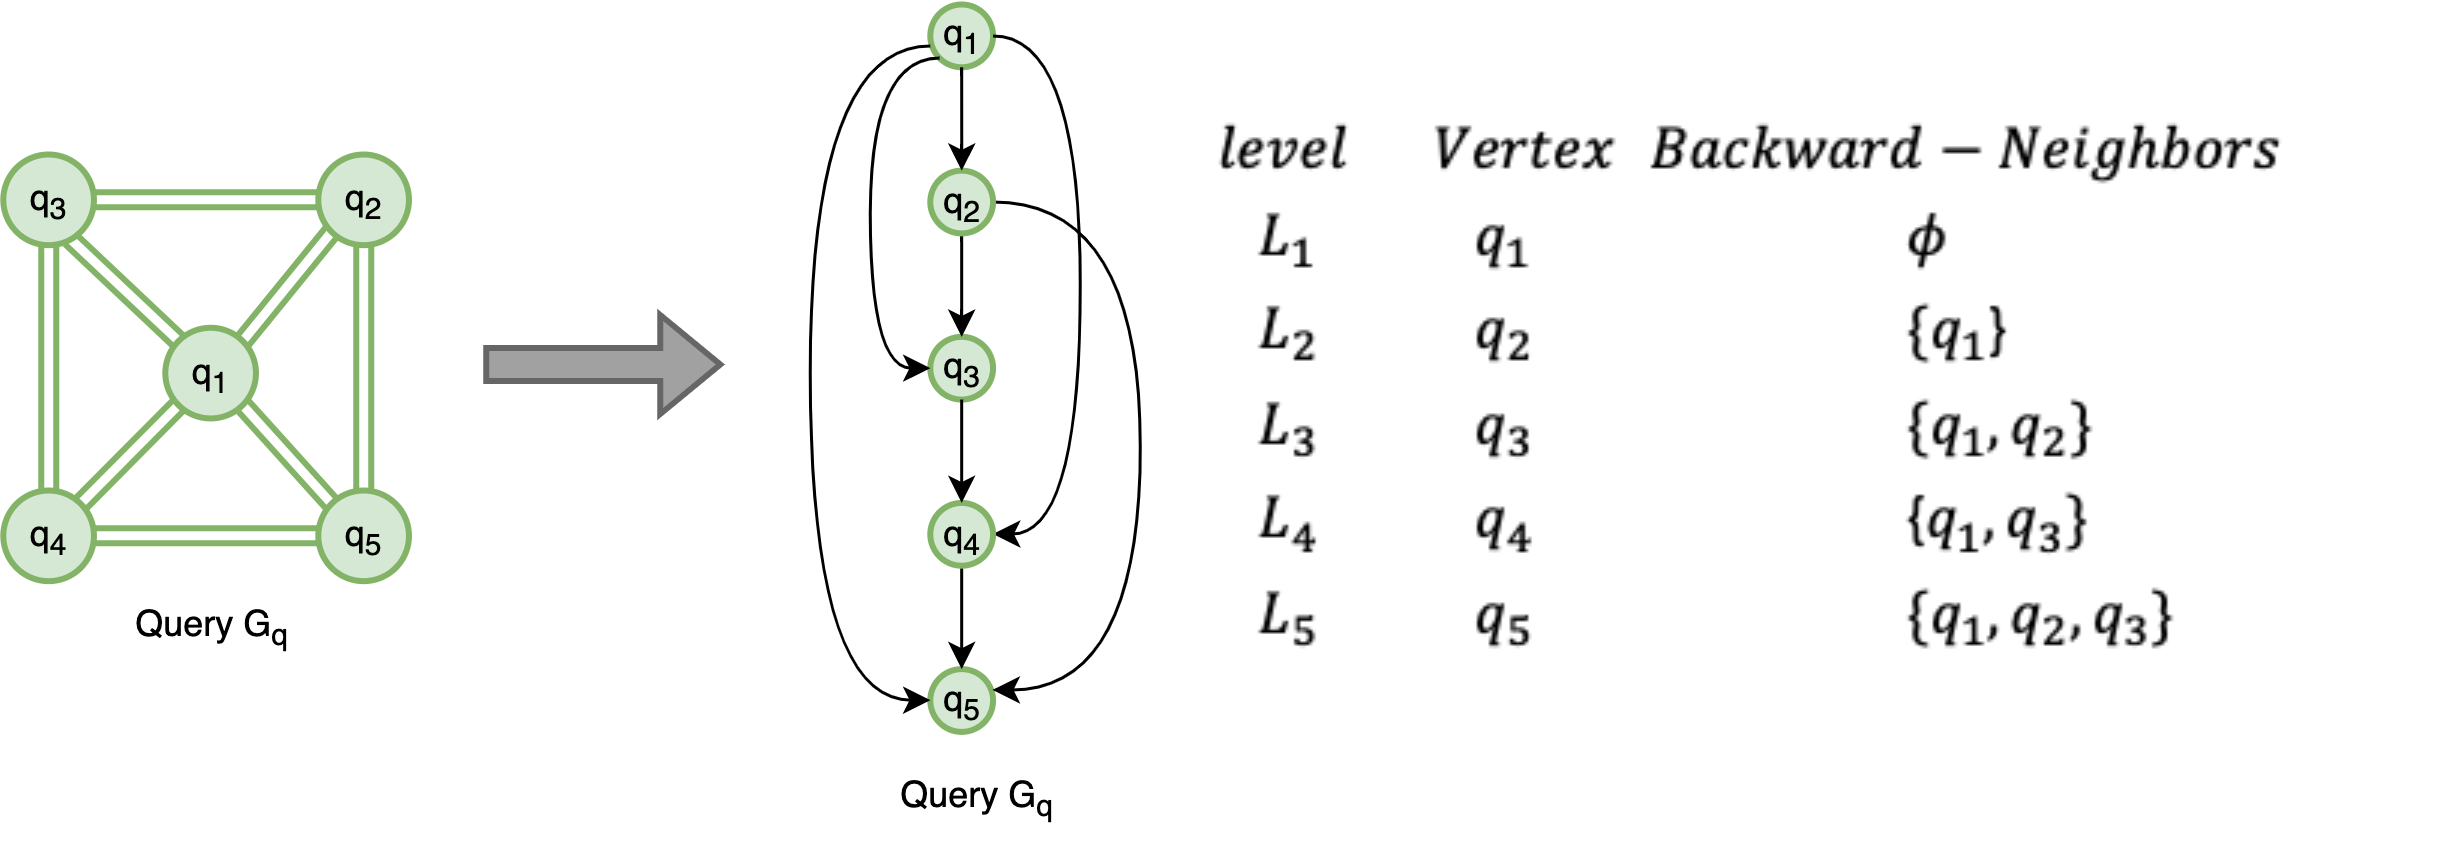
\includegraphics[width=\textwidth]{fig/LR/query-sequencing.png}
    \caption{Query Sequencing output of $G_q$ using \textit{VF3}}
    \label{fig:query-sequencing}
\end{figure}

\subsection{Symmetry Detection and Breaking}\label{sec:sym-detection}
Symmetry is the existence of automorphism in a graph. Automorphism, as the name suggests, is a graph that is isomorphic to itself.
An automorphism of a graph is a permutation of vertices that maintains edges and non-edges.
% Formally, an automorphism of a graph $G=(V,E)$ is  permutation $\sigma$ of the vertex set $V$ such that the pair of vertices $(u,v)$ form an edge if and only if $(\sigma(u), \sigma(v))$ also forms an edge.
The set of automorphic permutations of the vertex set is called the \textit{automorphism group}.
Figure \ref{fig:automorphism} shows the automorphism group of the query graph $G_q$.
\textit{Orbit} is an equivalence class of vertices in the automorphism group.
\begin{figure}
    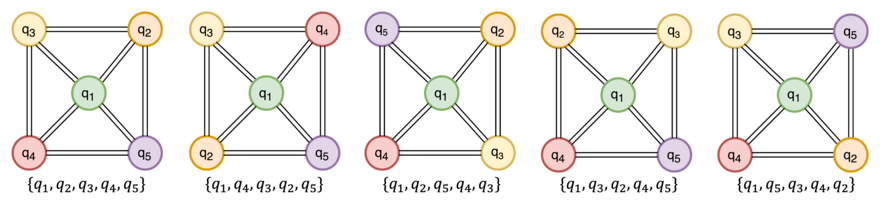
\includegraphics[width=\textwidth]{fig/LR/automorphism.png}
    \caption{Automorphism group of $G_q$}
    \label{fig:automorphism}
\end{figure}

The presence of symmetry essentially causes the same subgraph of the data graph to be counted multiple times which results in extra work.
The easiest technique that can be employed to avoid this is called symmetry breaking. This makes sure that the ties are resolved at the moment they are generated, hence avoiding redundant work.
An easy way to break symmetry is by having an order between the matches of data graph between the symmetric levels, which was introduced by \cite{symbreak}. Algorithm \ref{algo:symbrk} lists the pseudocode for detecting symmetry and generating ordering for symmetry based pruning. Note, the \texttt{GetAutomorphismGroup} and \texttt{GetOrbits} routines used here are provided by NAUTY \cite{nauty}.
% \RN{Where are the functions GetXYZ/}

\begin{algorithm}
    \caption{Symmetry breaking}
    \label{algo:symbrk}
    \SetKwFunction{gag}{GetAutomorphismGroup}
    \SetKwFunction{gorb}{GetOrbits}
    \KwIn{Template Graph, $G_q$}
    \KwOut{Set of partial node orderings, $\mathcal{P}_q$}
    $\mathcal{A} \leftarrow$ \gag{$G_q$}\;
    \While{$\mathcal{A} \neq \mathbb{I}$}{
        $\mathcal{O}_\mathcal{A} \leftarrow$ \gorb{$\mathcal{A}$}\;
        Pick largest orbit $\{v_1, v_2, \dots, v_k\}$ from $\mathcal{O}_\mathcal{A}$\;
        Add $v_1 < v_2, v_1 < v_3, \dots, v_1 < v_k$ to $\mathcal{P}_q$\;
        $\mathcal{A} \leftarrow \{\alpha | \alpha\in\mathcal{A}, \alpha(v_1) = v_1 \}$\;
    }
\end{algorithm}


For the query graph in Figure \ref{fig:sgm-example}, to avoid redundancy due to automorphism $\{q_1, q_4, q_3, q_2, q_5\}$ of $G_q$, it can be made sure that the data graph vertices matched at level 2 have labels less than the vertices matched at level 4. This is an example of \textit{lexicographic symmetry} breaking.
Another symmetry breaking order can be based on the degree of data graph nodes.
A key observation is that the symmetry breaking criteria can be different for different levels but not always different for different subtrees.
This will be formally established and utilized in Section \ref{sec:hy-symbreak}.

% \iffalse
%     \subsection{Reuse Detection}\label{sec:reuse-detection}
%     Set intersection operation for generating candidates at the next level is the most time-consuming operation in subgraph enumeration, this is a well-known fact in the literature and also re-verified in section \samiran{cite stacked bar graph figure}.
%     While traversing the search tree each node needs a set intersection operation on adjacency lists of backward neighbors (vertices matched with levels connected at the next level).
%     The number of backward neighbors at each level increases with increasing template size. This results in even more adjacency list intersections at each level.
%     RPS \cite{RPS-paper} reduces these operations by generating an intersection reuse plan, this plan smartly finds the intersections that will be required by more than one node and stores them when first calculated. There is a lot of intersection reuse possible with RPS as they employ a BFS strategy.
%     Similar reuse is not possible in DFS traversal since the past information is lost while backtracking.
%     However, Some levels of the sequenced query graphs have similar backward neighbor lists. For such queries' the majority of intersections can be reused by simply storing the intermediate intersection results. This technique is discussed in detail in Section \samiran{cite improvements section}.
%     To do this efficiently, the problem of finding level mappings with the most similar adjacency lists is posed as a linear programming optimization problem.

%     Let, the sequenced query graph be $G_q=(V_q, E_q)$ with $|V_q|=k$ and the vertex sequence $S_q$.
%     $\mathcal{N}(.)$ be the function for getting the backward neighbor list of a vertex.
%     For each pair of vertices at level $i$ and $j$ let $W_{ij}$ be a measure of the commonality between their backward neighbors' lists. Let $X_{i,j}$ be the decision variable which tells if vertex $i$ should reuse intersections from vertex $j$.

%     With these definitions the optimization problem can be modelled as:
%     \begin{align}
%         \max \sum_{i=j+1}^{k}\sum_{j=1}^{k} W_{ij} X_{ij} \\
%         \text{s.t.}
%         \sum_{j=1}^k X_{ij} \leq 1. \quad \forall i \in \{1, \dots, k\}
%     \end{align}
%     Where, $$
%         W_{ij} = \begin{cases}
%             |\mathcal{N}(S_q[i]) \cap \mathcal{N}(S_q[j])| \qquad \text{if} \quad i>j, \mathcal{N}(S_q[i]) \supseteq \mathcal{N}(S_q[j]) \\
%             0   \qquad \text{Otherwise}
%         \end{cases}
%     $$
%     This problem is a linear semi-assignment problem (LSAP) with the optimal solution being the greedy solution itself.
%     This is easy to establish as any other solution can be improved by switching to the greedy solution.
%     The solution to this problem is:
%     $$
%         X_{ij}=\begin{cases}
%             1   \qquad \text{if } j=\argmax_j(w_{ij}>0); \\
%             0   \qquad \text{Otherwise}
%         \end{cases}
%     $$

%     Reuse detection involves a find minimum operation for each level in $G_q$ hence it is polynomial time and can be performed on CPU for small-sized query graphs. Once, this is performed, it gives the levels that are \textit{reusable}. The intersection results for these levels are to be stored, this is discussed in detail in Section \ref{sec:reuse-impl}.

%     \newpage
% \fi

\section{Data Graph Preprocessing}\label{graph-preprocessing}

Data graph preprocessing involves operations on the data graph to shrink the search tree during traversal.
With GPU implementations, preprocessing also helps to improve coalesced memory accesses and memory utilization.


\subsection{Peeling}\label{peeling}
Subgraph Enumeration produces isomorphic matches of the query graph in the data graph.
Naturally, each match needs to have degree greater than the degree of the corresponding query node.
This implies that: \textit{Vertices in data graph with degree less than minimum query degree will never form any matches.}
Using this simple observation, all vertices with degree lesser than the minimum query degree can be deleted from the data graph.
This can be done iteratively as the observation holds for the resulting data graph.
This process is known as \textit{Peeling}.
Empirical experiments conducted by \cite{PARSEC_VD} show that \textit{Peeling} should be performed till at most $5\%$ of nodes are deleted.
Algorithm \ref{algo:peel} shows the peeling routine.
% Note the filtering of vertices is done on GPU using the CUB library \cite{cub}.
\begin{algorithm}[h]
    \caption{Peeling data graph}
    \label{algo:peel}

    \SetKwData{nfs}{PrunedVertices}
    \SetKwData{efs}{PrunedEdges}
    \SetKwFunction{d}{Degree}

    \KwIn{ Minimum query graph degree, $d_{q,min}$, $G_d = (V_d, E_d)$:}
    \Repeat{$|\nfs| < 0.05 \times |V_d|$}{
        \nfs $\leftarrow \{u | u \in V_d, \d{u} < d_{q,min}\}$\;
        \If{$|\nfs| = 0$}{\text{Break;}}
        $\efs \leftarrow \{(u, v) | u \textbf{ or } v \in \nfs  $\;
        $V_d \leftarrow V_d \setminus \nfs$\;
        $E_d \leftarrow E_d \setminus \efs$\;
    }
\end{algorithm}
\begin{figure}
    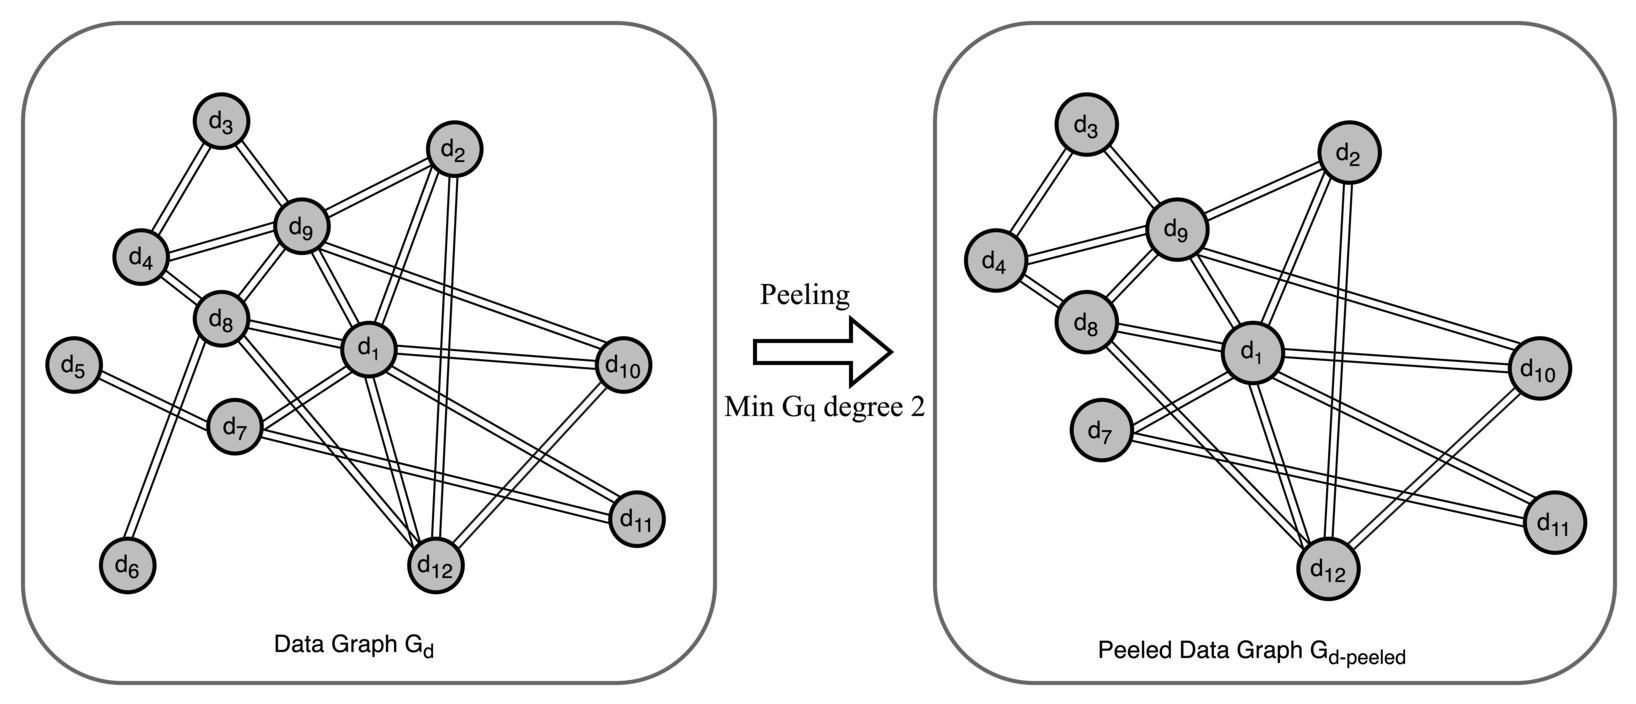
\includegraphics[width=\textwidth]{fig/LR/peeling.png}
    \caption{Peeling Example}
    \label{fig:peeling}
\end{figure}

\subsection{Priority Sorting}\label{sec:prio-sorting}
CSRCOO storage format allows efficient storage of graphs in CPU memory.
As mentioned in Section \ref{storage-format}, the \textit{Column Index} array is sorted by vertex labels to enable binary search.
However, efficient symmetry breaking demands the neighbors be listed in a different order.
To achieve this, we need another copy of the \textit{Column Index} array in a \textit{priority} sorted fashion while maintaining the \textit{Row Pointer} boundaries. This array is referred to as \textit{Priority Sorted Column Index} or \textit{PSCI}.
The \textit{priority} can be any property of the vertices; in our case two properties are explored: Degree and Degeneracy.
\begin{figure}
    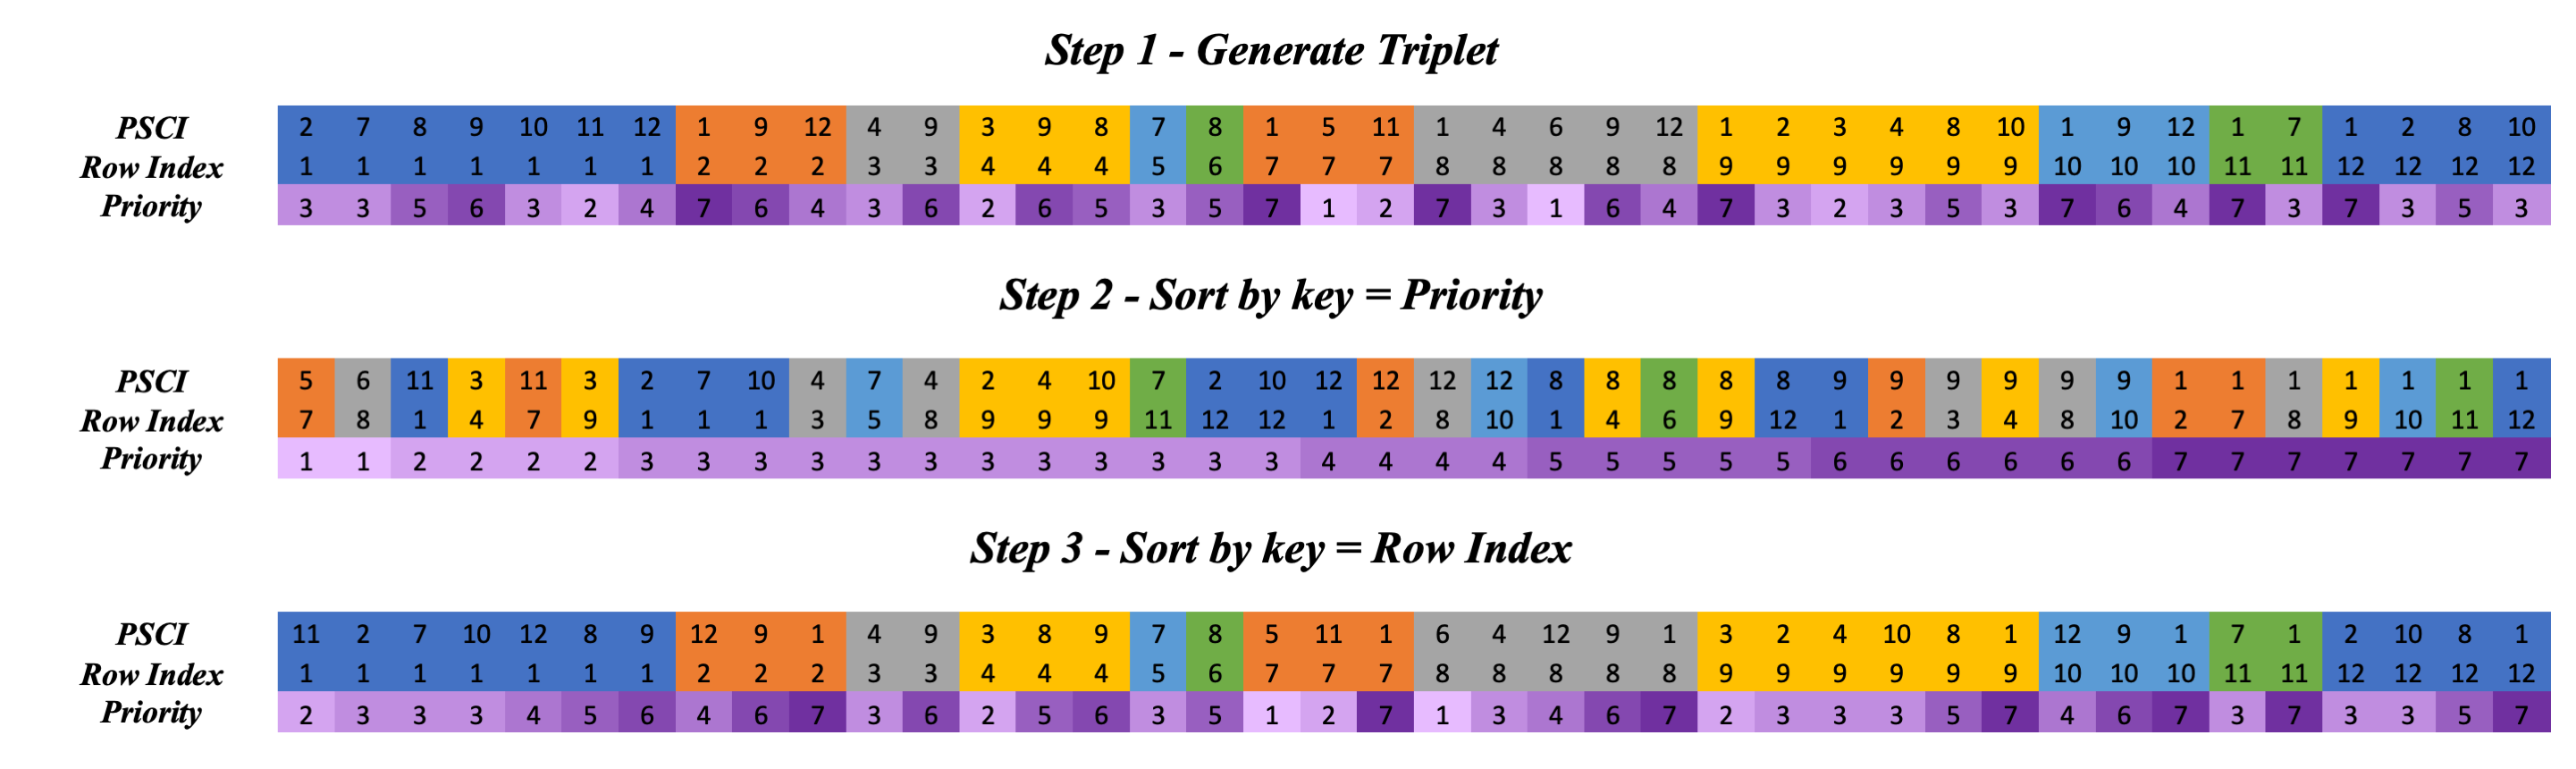
\includegraphics[width=\textwidth]{fig/LR/prio-sorting.png}
    \caption{Generating Priority Sorted Column Index Array}
    \label{fig:prio-sorting}
\end{figure}
Given the size of data graph, GPUs are used for this preprocessing task.
% GPUs are used for this sorting task as data graphs are significantly large.
The \textit{PSCI} array can be generated using a series of two stable sorts. 
% Since sorting is fast on GPUs, it can be achieved by using the CUB library \cite{cub}.
Sorting can be efficiently executed on GPUs using the CUB library \cite{cub}.
To start with, the \textit{PSCI} array is taken as a copy of the original \textit{Column Index} array.
An array of triplets is created with each entry containing an element from \textit{PSCI}, \textit{Row Index}, and \textit{priority}. 
Here, \textit{priority} is an array populated with the entries corresponding to the required vertex property in \textit{PSCI}.
This array of triplets is subjected to two key-based stable sorts, the first sort is with the keys being entries in the \textit{priority} array while the second sort is with the keys being entries in the \textit{Row Index} array. Figure \ref{fig:prio-sorting} shows the priority sorting performed on $G_d$ as a series of key sorts.

\subsection{Induced Subgraph}\label{encoding}
Search space in the subgraph enumeration problem is essentially the whole graph for a general query.
This makes the problem extremely challenging to scale.
However, most practical applications of subgraph isomorphism focus on dense templates.
As explored in \cite{mohammad_K-clique}, restricting the search space can provide immense performance improvements.
\begin{figure}
    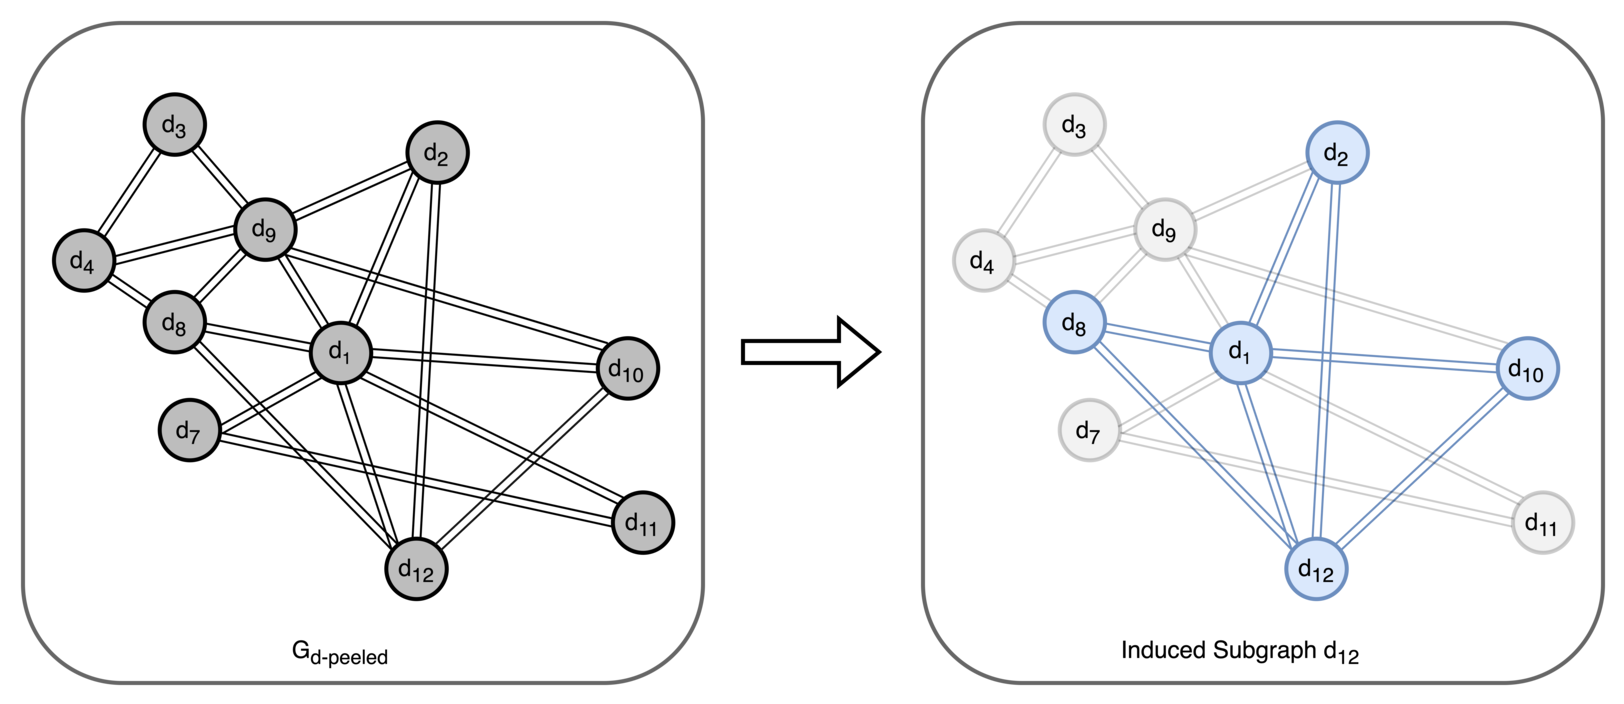
\includegraphics[width=\textwidth]{fig/LR/Induced-subgraph.png}
    \caption{Induced Subgraph for vertex $d_{12}$}
    \label{fig:induced-subgraph}
\end{figure}
The search space can be restricted by focusing on query graphs containing at least one \textit{central node}.
A central node is defined as a node in the query graph that is connected to all other nodes.
Under the assumption of a central node, the search space for each match can be limited to the subgraph induced by the data graph vertex matched to the central node.
Figure \ref{fig:induced-subgraph} shows the subgraph induced by vertex $d_{12}$.
To save storage space and perform fast adjacency list intersections, the induced subgraph is stored in a binary adjacency matrix format.
% The binary format allows fast set intersection operations as well as efficient symmetry breaking \cite{mohammad_K-clique}.
The columns of the adjacency matrix are ordered according to the \textit{Priority Sorted Column Index} array to enable efficient symmetry breaking.

\section{Search Tree Traversal}\label{DFS-T}
% The algorithm was first developed by \cite{ullman_sgm} in $1976$.
% This was a DFS based brute force search technique that uses an adjacency matrix of size $|V_q| \times |V_d|$ as a bijection between an element in the query template and data graph.
% These matrices are recursively generated in a DFS based enumeration process to ultimately generate all the instances.
% The new candidates are generated using the conditions imposed by query graph itself.
% This algorithm assumes a directed query graph and template graph as input.
This section explains how the sequenced query graph $G_q$ and processed data graph $G_d$ are used to perform the search tree traversal for enumerating all matches.
% Let, the directed acyclic query graph be ${G}_q = (V_q, E_q)$ and the processed data graph be $G_d=(V_d, E_d)$.
% We will assume this transformation for the example given in Figure \ref{fig:sgm-example}, the post process query graph is shown in \ref{fig:query-sequencing} and data graph is shown in Figure \ref{fig:peeling}.\\

\begin{algorithm}
    \caption{DFS Traversal}
    \label{algo:DFS-traversal}
    \small
    \SetKwData{l}{$l_{init}$}
    \SetKwData{isubgraph}{$G^d_{ind}$}
    \SetKwData{imatches}{$\texttt{matches}_{init}$}
    \SetKwData{isize}{$\texttt{num\_matches}_{init}$}
    \SetKwData{currIdx}{$\texttt{curr\_idx}$}
    \SetKwData{matches}{$\texttt{matches}$}
    \SetKwData{nmatches}{$\texttt{num\_matches}$}

    \SetKwFunction{intersect}{GenNextCandidates}

    \SetKwData{omatches}{$\texttt{final\_enum}$}
    \SetKwData{ocount}{$\texttt{count}$}

    \KwIn{Sequenced Query Graph: $G_q=(V_q,E_q), S_q$ \newline
        Induced Subgraph: \isubgraph. Initial level: \l \newline
        Initial set of Nodes at \l: \imatches and size \isize
    }
    \KwOut{Set of enumerated matches and count: \omatches, \ocount}
    $l \leftarrow $ \l, $\matches[l] \leftarrow $\imatches, $\nmatches[l] \leftarrow $\isize\;
    $ \currIdx \leftarrow 0$, $\omatches \leftarrow \phi $, $\ocount \leftarrow 0$  \;
    \While{$\currIdx[l] \leq \nmatches[l] $}{

        % $\matches[l+1] \leftarrow \matches[l][\currIdx[l]]$\;
        \intersect()\;
        $\nmatches[l+1]=|\matches[l+1]|$\;
        \If{$(\nmatches > 0 \textbf{ and } l < |V_q|-1$)}{
            $l\leftarrow l+1$\;
            $\currIdx[l]\leftarrow 0$\;
        }
        \ElseIf{$l==|V_q|-1$}{
            \For{$n=\l \textbf{ to } \nmatches[l+1]$}{
                $\texttt{match}\leftarrow \phi$\;
                \For{$k=\l \textbf{ to } l$}{
                    $\texttt{match} \leftarrow \texttt{match} \cup \matches[k][\currIdx[k]]$
                }
                $\omatches \leftarrow \omatches \cup \texttt{match}$
            }
            $\ocount\leftarrow \ocount + \nmatches[l+1]$
        }
        \Else{
            $\currIdx[l]\leftarrow \currIdx[l]+1$\;
            \While{$\currIdx[l]==\nmatches[l] \textbf{ and } l > \l$ }{
                $l\leftarrow l-1$\;
                $currIdx[l]\leftarrow \currIdx[l] +1 $\;
            }
        }

    }
\end{algorithm}

Algorithm \ref{algo:DFS-traversal} describes the DFS-based iterative search tree traversal.
The whole traversal can work within a DFS stack of size $|V_q|\times Degree_{max}(G_d)$.
\texttt{GetNextNodes} function is called at each node of the search tree which generates the candidates to be visited at the next level.
This function is listed in Algorithm \ref{algo:intersect}.
It performs an adjacency list intersection operation to generate all possible candidates for the next level (lines 2 - 5).
The next loop, (lines 6-8) prunes redundant candidates which are generated due to the symmetry in $G_q$.
Note that, the $\mathcal{V}_{orient}$ set used in Algorithm \ref{algo:intersect} is directly available from the binary adjacency matrix generated in Section \ref{encoding}.

\begin{algorithm}
    \caption{Generate Candidates for Next Level}
    \label{algo:intersect}
    \SetKwData{isubgraph}{$G^d_{ind}$}
    \SetKwData{currIdx}{$\texttt{curr\_idx}$}
    \SetKwData{matches}{$\texttt{matches}$}
    \SetKwData{nmatches}{$\texttt{num\_matches}$}
    \SetKwFunction{intersect}{GenNextCandidates}
    \KwIn{Induced Subgraph \isubgraph, level $l$ \newline
        Backward Neighbor List $\mathcal{N'}$ \newline
        Symmetry levels List $\mathcal{S}$ \newline
        Set of vertices of lower priority than given vertex $\mathcal{V}_{orient}()$ \newline
        List of matches in previous levels $\matches[]$
    }
    $\texttt{Function }\intersect() $\newline
    \While{$(\currIdx[l]<\nmatches[l])$}{
    \ForAll{$k \in \mathcal{N'}(S_q[l+1])$}{
        $u \leftarrow \matches[k][\currIdx[k]]$\;
        $\matches[l+1] \leftarrow \matches[l+1]\cap \mathcal{N}(\isubgraph(u))$\;
        }
        \ForAll{$j \in \mathcal{S}(S_q[l+1])$}{
            $u \leftarrow \matches[j]$\;
            $\matches[l+1]\leftarrow \matches[l+1] \setminus \mathcal{V}_{orient}(u)$\;
        }
    }
    $\texttt{Function End}$
\end{algorithm}

We now walk through the search tree traversal algorithm with the example query graph sequence from Figure \ref{fig:query-sequencing} and the peeled data graph in Figure \ref{fig:peeling}.
% Note, the pseudocode gives a DFS-based traversal tree but since it does not store the whole tree, we resort to a BFS traversal here for enumerating the whole exploration tree. \RN{language!}
Note, the pseudocode in Algorithm \ref{algo:DFS-traversal} describes DFS-based traversal while the example enumerates search tree traversal in BFS manner for illustration purposes.

\begin{enumerate}[Step 1:]
    \item Select candidates in $G_d$ with degree greater than or equal to $q_1$. In this example, vertices $\{d_1, d_8, d_9, d_{12}\}$ will be selected. All of them are matched to $q_1$ and traversed separately. For conciseness, only $d_1$ and $d_{12}$ are considered. The matches are shown in Figure \ref{fig:sgm-step1}.
          \begin{figure}
              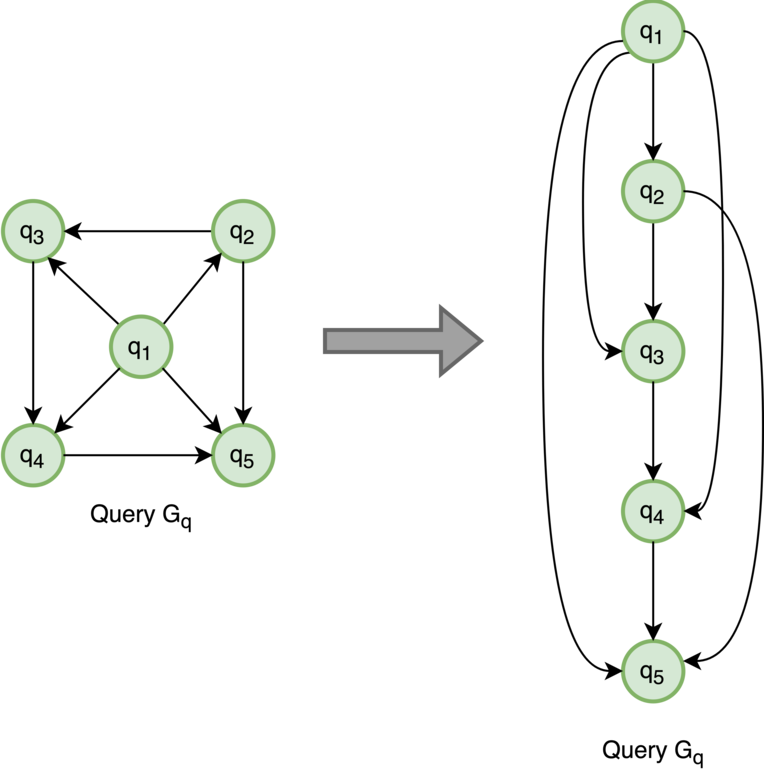
\includegraphics[width=\textwidth]{fig/LR/sgm-step1.png}
              \caption{Step 1}
              \label{fig:sgm-step1}
          \end{figure}
    \item For candidates at level 2, select all neighbors of the vertex matched at level 1 with degree greater than $d(q_2)$, i.e., 3. As shown in Figure \ref{fig:sgm-step2}, there will be 6 candidates: $\{d_2, d_7, d_8, d_9, d_{10}, d_{12}\}$ in the subtree rooted at $d_1$. 
    $d_7$ is pruned out of these 6 candidates since it has degree less than $q_2$.\\
          \begin{figure}
              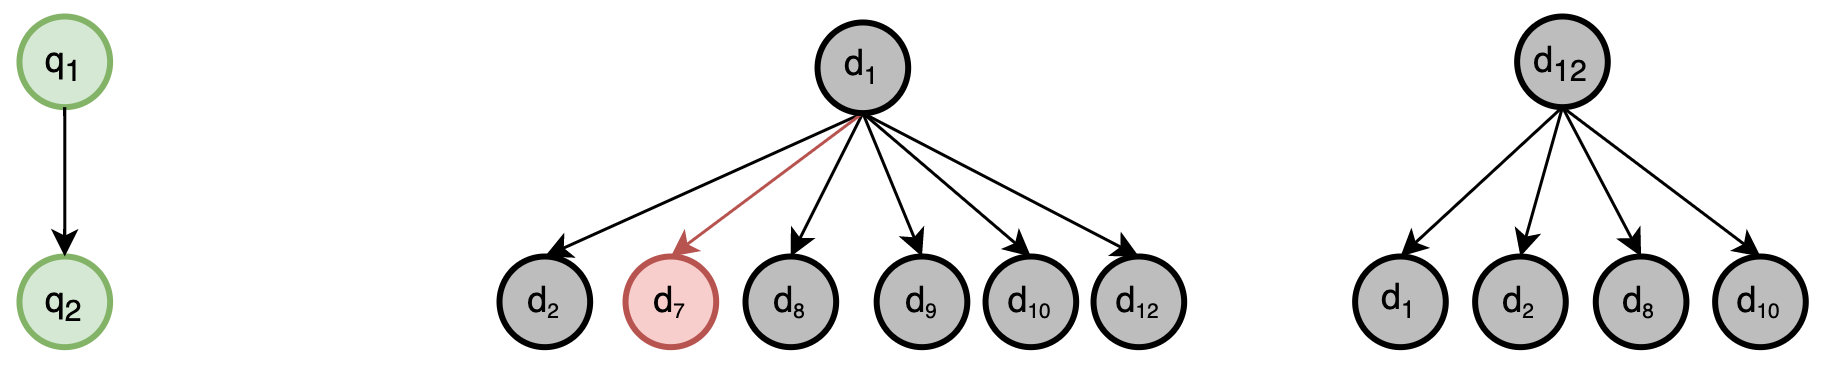
\includegraphics[width=\textwidth]{fig/LR/sgm-step2.png}
              \caption{Step 2}
              \label{fig:sgm-step2}
          \end{figure}
          For the subtree rooted at $d_{12}$, there will be 4 candidates: $\{d_1, d_2, d_8, d_{10}\}$ and none can be pruned.
    \item Level 3 candidates are obtained by the adjacency list intersection of matches at level 2 and level 1. 
    Since this level is symmetric to level 2, symmetry breaking needs to be performed. Decreasing degree criteria for symmetry breaking is used in this example.
          \begin{figure}
              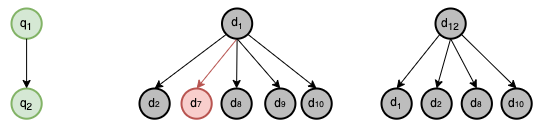
\includegraphics[width=\textwidth]{fig/LR/sgm-step3.png}
              \caption{Step 3}
              \label{fig:sgm-step3}
          \end{figure}
          Figure \ref{fig:sgm-step3} shows all candidates at level 3. 
          The candidates marked in red are pruned.
          For example, $d_9$ is pruned due to symmetry breaking in the subtree (${d_1, d_8, \dots}$) since $Degree(d_9) > Degree(d_8)$. 
          Ties are resolved using the lexicographic criterion.
    \item For level 4 candidates, the adjacency list intersection of vertices matched at $q_1$ and $q_3$ is required. This level is also symmetric to level 2.
          As illustrated in Figure \ref{fig:sgm-step4}, the subtree rooted at $d_{12}$ does not yield any candidates.\\
          The other subtree gets two candidates for ($d_1, d_8, d_{12}, \dots $). and one candidate each for the remaining subtrees.
          $d_9$ is pruned due to symmetry breaking.
          \begin{figure}
              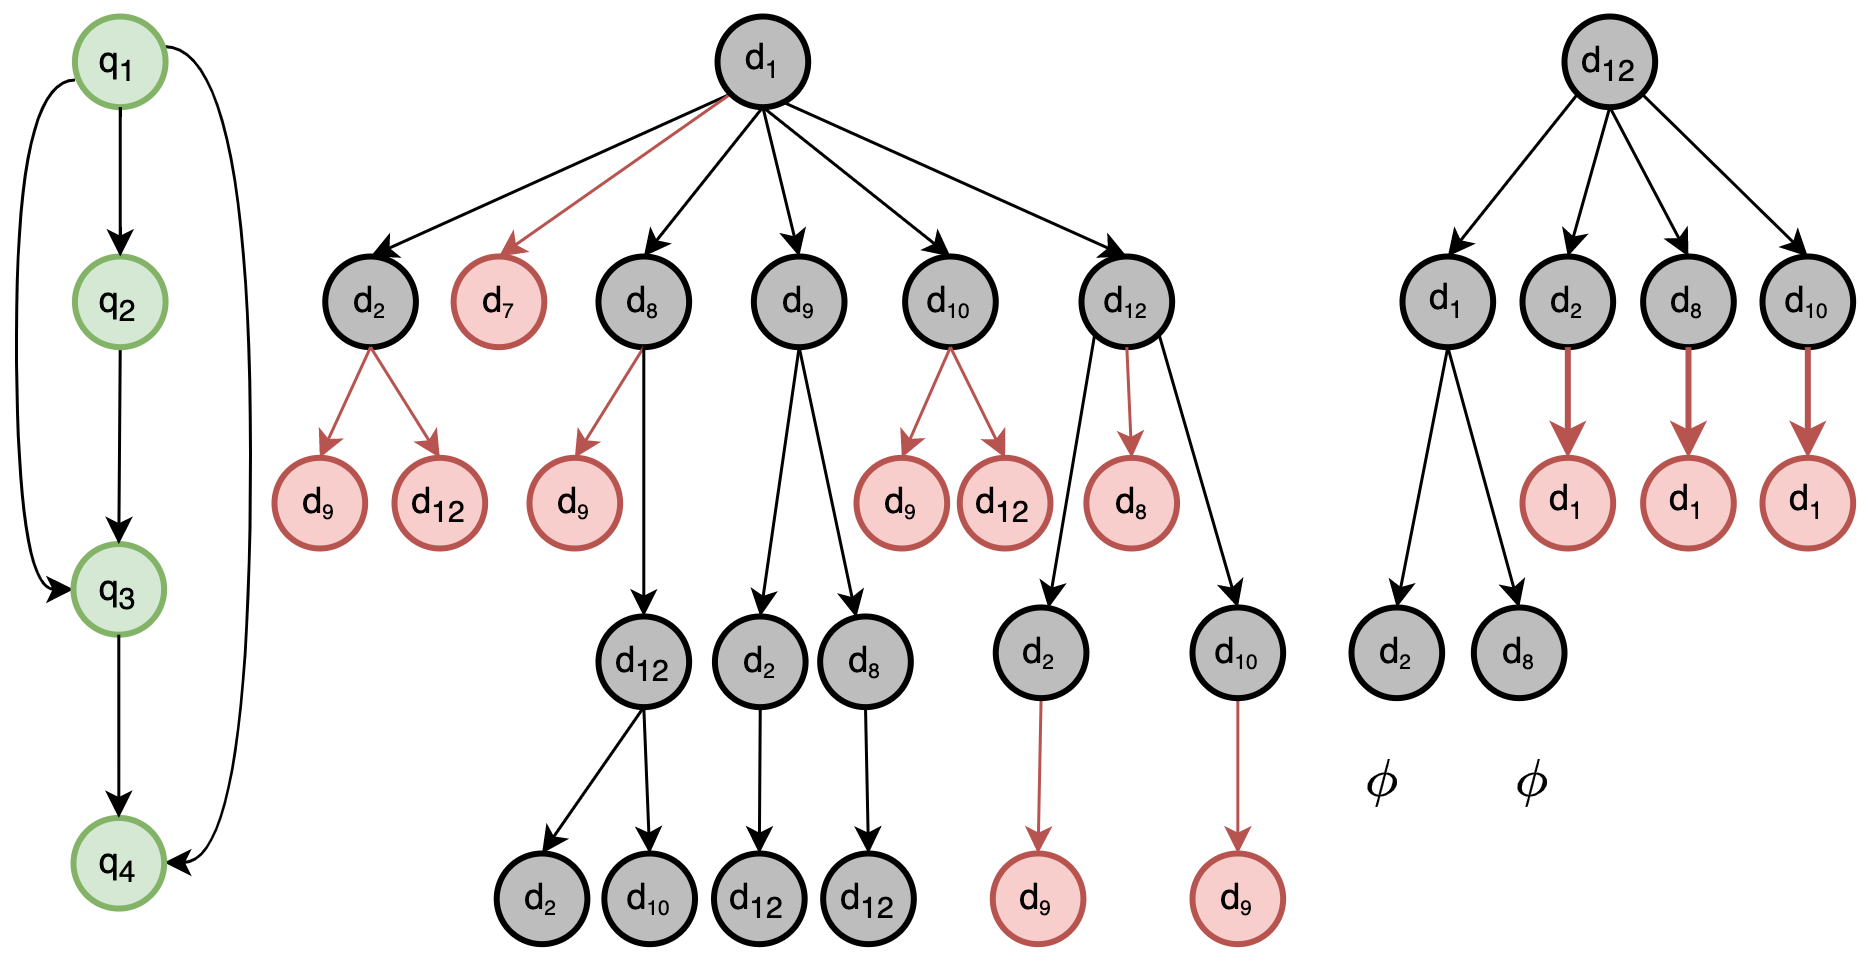
\includegraphics[width=\textwidth]{fig/LR/sgm-step4.png}
              \caption{Step 4}
              \label{fig:sgm-step4}
          \end{figure}
    \item Level 5 candidates (or final matches) are generated by the adjacency list intersection of matches at $q_1$, $q_2$, and $q_4$. This level is symmetric to both $q_2$ and $q_3$.
          The candidates generated by intersection at the first leg are $\{d_8, d_{10}\}$, symmetry breaking will eliminate $d_8$ as $Degree(d_8)>Degree(d_2)$.
          There is a tie between $d_2$ and $d_{10}$ which is resolved lexicographically.
          \begin{figure}
          \centering
              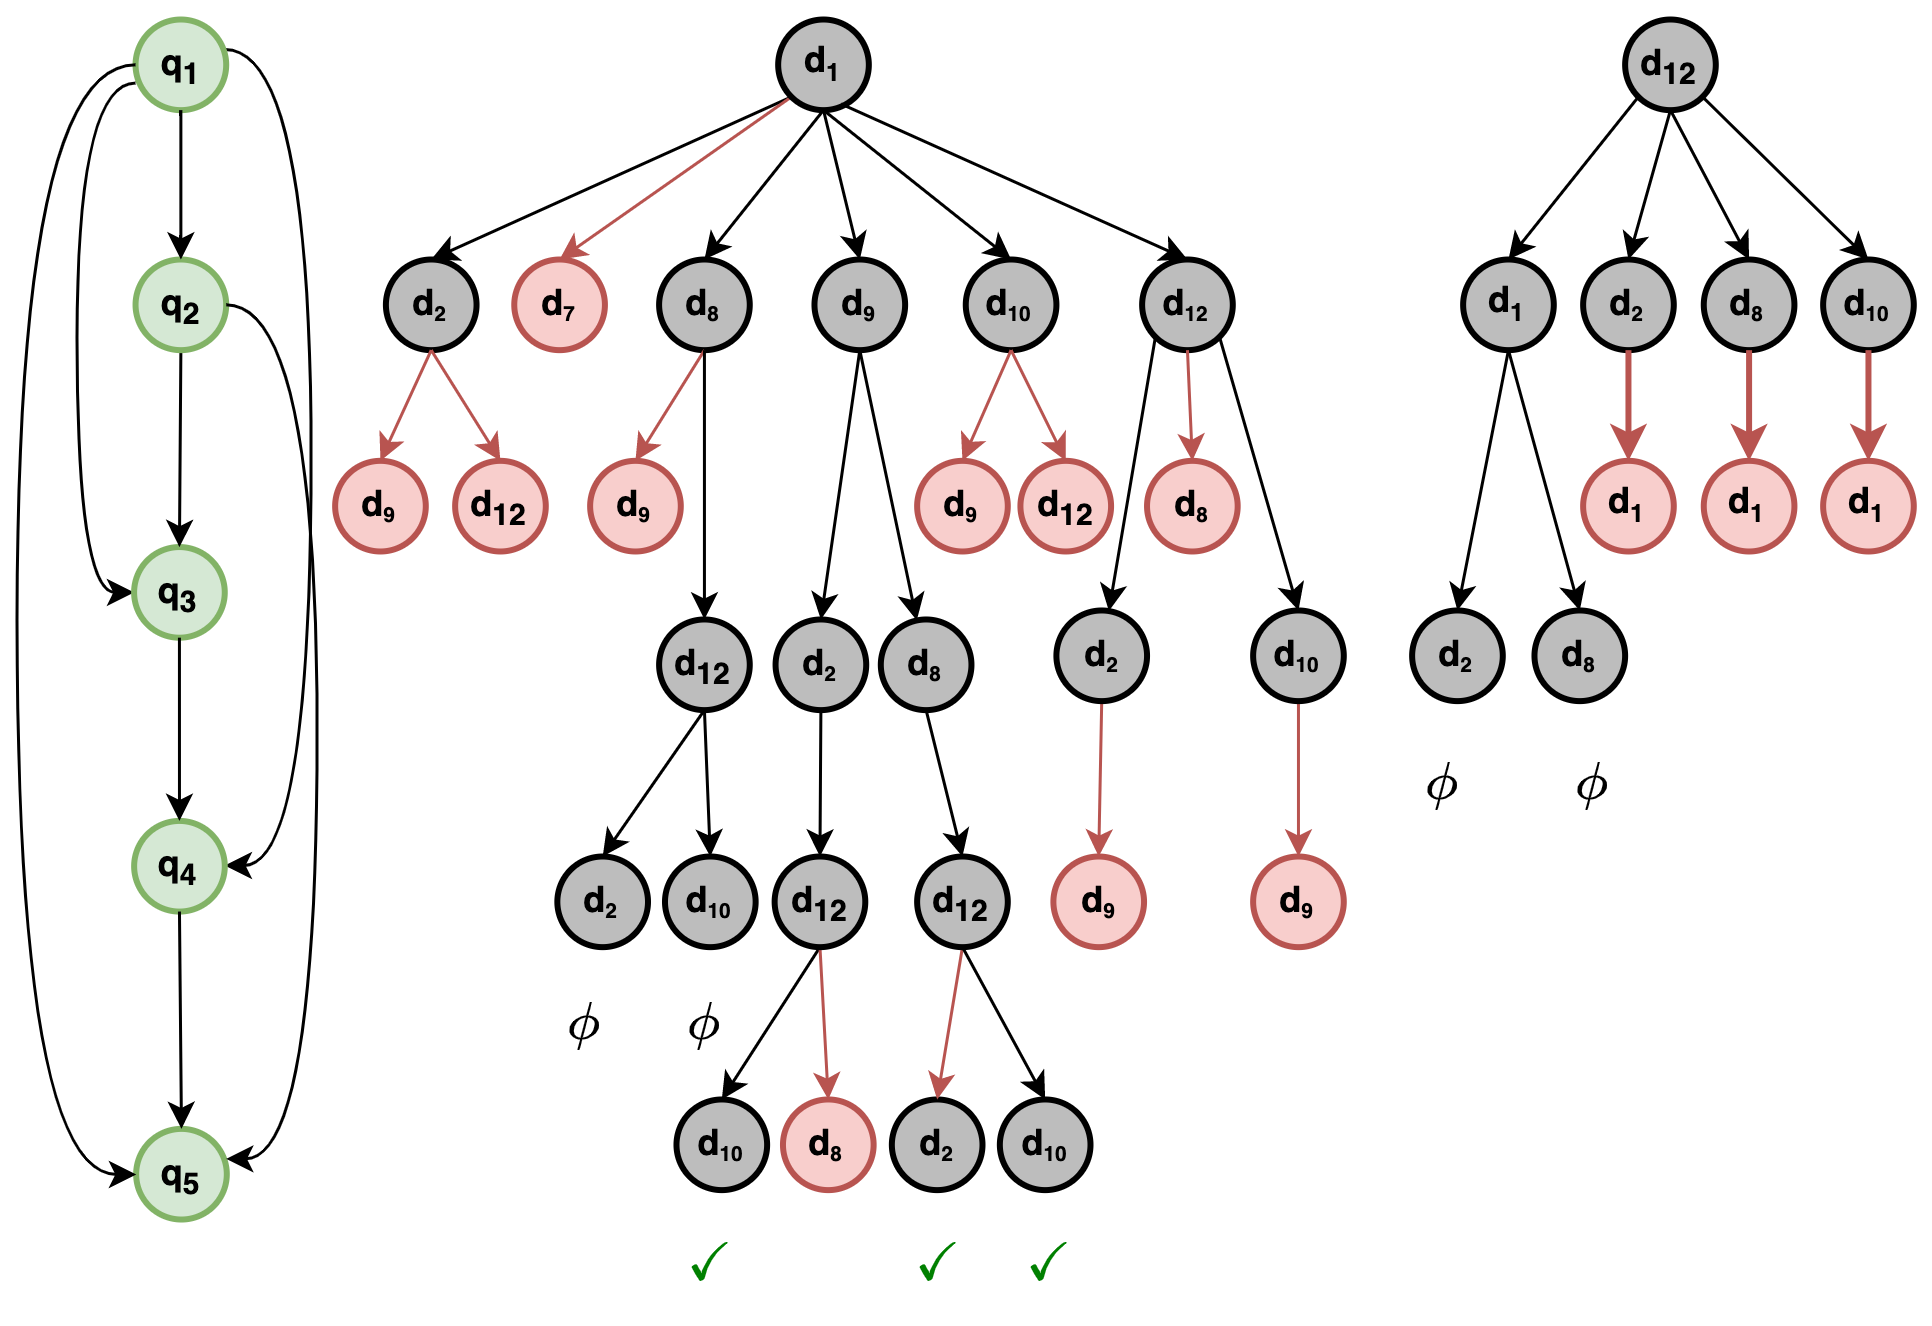
\includegraphics[width=0.9\textwidth]{fig/LR/sgm-step5.png}
              \caption{Step 5}
              \label{fig:sgm-step5}
          \end{figure}
          Similarly, the other leg generates two more candidates for level 5.
\end{enumerate}
This way the search tree traversal process terminates with final matches
$\{d_1, d_9, d_2, d_{12}, d_{10} \}, \{d_1, d_9, d_8, d_{12}, d_2\}$, and $\{d_1, d_9, d_8, d_{12}, d_{10}\}$.
There might be other matches originating from the subtrees rooted at $\{d_8, d_9\}$ which were not illustrated here.

To conclude, this chapter provides a detailed understanding of all techniques involved in subgraph enumeration. As we can see, all subtrees are independent of each other therefore they can be easily parallelized on GPUs.

One subtle observation to be made here is that the exploration is dependent on the symmetry breaking criteria.
We can see from Figure \ref{fig:sgm-step4} that there would be many more candidates at level 4 if symmetry breaking was performed using lexicographic or increasing degree criterion.
These candidates would have ultimately pruned in lower levels, resulting in extra work.
Therefore, selecting an efficient symmetry-breaking strategy is important; it is thoroughly discussed in Section \ref{sec:hy-symbreak}.
